\documentclass[10pt,twocolumn]{article}
% Shared two-column preamble for the three research papers.
% Use with: \documentclass[10pt,twocolumn]{article}
% Then in main.tex: % Shared two-column preamble for the three research papers.
% Use with: \documentclass[10pt,twocolumn]{article}
% Then in main.tex: % Shared two-column preamble for the three research papers.
% Use with: \documentclass[10pt,twocolumn]{article}
% Then in main.tex: \input{../../shared/latex/twocolumn_preamble.tex}

\usepackage[margin=0.75in]{geometry}
\usepackage[utf8]{inputenc}
\usepackage[T1]{fontenc}
\usepackage{lmodern}
\usepackage{microtype}
\usepackage{amsmath,amssymb,amsthm}
\usepackage{graphicx}
\usepackage{booktabs}
\usepackage{caption}
\usepackage{subcaption}
\usepackage{hyperref}
\usepackage{url}
\usepackage{xcolor}
\usepackage{algorithm}
\usepackage{algorithmic}
\usepackage{multirow}
\usepackage{titlesec}
\usepackage{authblk}

\hypersetup{colorlinks=true,linkcolor=blue!50!black,citecolor=blue!50!black,urlcolor=blue!50!black}

\titleformat{\section}{\normalfont\large\bfseries}{\thesection}{0.6em}{}
\titleformat{\subsection}{\normalfont\bfseries}{\thesubsection}{0.5em}{}

\captionsetup{font=small,labelfont=bf,skip=4pt}
\setlength{\columnsep}{0.25in}
\setlength{\parskip}{2pt}

\newtheorem{theorem}{Theorem}
\newtheorem{proposition}[theorem]{Proposition}
\newtheorem{definition}[theorem]{Definition}


\usepackage[margin=0.75in]{geometry}
\usepackage[utf8]{inputenc}
\usepackage[T1]{fontenc}
\usepackage{lmodern}
\usepackage{microtype}
\usepackage{amsmath,amssymb,amsthm}
\usepackage{graphicx}
\usepackage{booktabs}
\usepackage{caption}
\usepackage{subcaption}
\usepackage{hyperref}
\usepackage{url}
\usepackage{xcolor}
\usepackage{algorithm}
\usepackage{algorithmic}
\usepackage{multirow}
\usepackage{titlesec}
\usepackage{authblk}

\hypersetup{colorlinks=true,linkcolor=blue!50!black,citecolor=blue!50!black,urlcolor=blue!50!black}

\titleformat{\section}{\normalfont\large\bfseries}{\thesection}{0.6em}{}
\titleformat{\subsection}{\normalfont\bfseries}{\thesubsection}{0.5em}{}

\captionsetup{font=small,labelfont=bf,skip=4pt}
\setlength{\columnsep}{0.25in}
\setlength{\parskip}{2pt}

\newtheorem{theorem}{Theorem}
\newtheorem{proposition}[theorem]{Proposition}
\newtheorem{definition}[theorem]{Definition}


\usepackage[margin=0.75in]{geometry}
\usepackage[utf8]{inputenc}
\usepackage[T1]{fontenc}
\usepackage{lmodern}
\usepackage{microtype}
\usepackage{amsmath,amssymb,amsthm}
\usepackage{graphicx}
\usepackage{booktabs}
\usepackage{caption}
\usepackage{subcaption}
\usepackage{hyperref}
\usepackage{url}
\usepackage{xcolor}
\usepackage{algorithm}
\usepackage{algorithmic}
\usepackage{multirow}
\usepackage{titlesec}
\usepackage{authblk}

\hypersetup{colorlinks=true,linkcolor=blue!50!black,citecolor=blue!50!black,urlcolor=blue!50!black}

\titleformat{\section}{\normalfont\large\bfseries}{\thesection}{0.6em}{}
\titleformat{\subsection}{\normalfont\bfseries}{\thesubsection}{0.5em}{}

\captionsetup{font=small,labelfont=bf,skip=4pt}
\setlength{\columnsep}{0.25in}
\setlength{\parskip}{2pt}

\newtheorem{theorem}{Theorem}
\newtheorem{proposition}[theorem]{Proposition}
\newtheorem{definition}[theorem]{Definition}

\newcommand{\BestDiscreteName}{discrete\_2}
\newcommand{\BestDiscreteAcc}{0.546}
\newcommand{\BestDiscreteLatency}{0.011}
\newcommand{\FastestEquivOdeName}{euler\_2}
\newcommand{\FastestEquivOdeAcc}{0.546}
\newcommand{\FastestEquivOdeLatency}{0.014}
\newcommand{\OdeSpeedup}{0.84}
\newcommand{\OdeLossRange}{0.053}
\newcommand{\DiscreteLossRange}{22.896}


\title{Continuous-Depth Transformers as Anytime Inference:\\
A Latency--Robustness Trade-off Study}
\author[1]{Luis Benvenuto}
\affil[1]{Data Science \& Mathematics, Independent Research}
\date{\today}

\begin{document}
\twocolumn[\maketitle
\begin{@twocolumnfalse}
\begin{abstract}
\noindent We treat the depth of a transformer as a continuous variable by
parameterising a single block as the vector field of an ordinary
differential equation (Neural ODE). At inference time, depth becomes a
solver-budget choice rather than an architectural constant. We compare
this Neural-ODE transformer against discrete-depth baselines on a
synthetic copy task across seven solver configurations and three discrete
depths. The headline result is the \emph{robustness} of continuous depth:
across solver configurations, the next-token cross-entropy varies by only
$\OdeLossRange$ nats, whereas a discrete model run at depths different
from its training depth diverges by $\DiscreteLossRange$ nats. Continuous
depth therefore enables a form of anytime inference that discrete depth
does not, even when raw latency parity is close.
\end{abstract}
\vspace{1em}
\end{@twocolumnfalse}]

\section{Introduction}
A transformer of $L$ layers is conventionally an architectural commitment:
once trained, it is also evaluated at $L$ layers. The Neural Ordinary
Differential Equation (Neural ODE) framework~\cite{chen2018node} suggests
an alternative: a single block $f_\theta$ defines a vector field, and the
forward pass solves
\begin{equation}
\frac{dh}{dt}=f_\theta(h),\quad h(0)=\text{embed}(x),\quad h(1)=\text{logits}.
\end{equation}
The number of function evaluations (NFE) becomes a solver budget chosen at
inference time. We ask:
\begin{quote}\emph{Does a continuous-depth transformer obtain a more
favourable latency/accuracy trade-off than discrete-depth baselines, or
at least a more robust one?}\end{quote}

\paragraph{Findings.} On a synthetic copy task, both formulations reach
similar accuracy. The crucial difference is robustness to inference-time
budget: across seven solver settings the ODE next-token cross-entropy
varies by only $\OdeLossRange$ nats; discrete depth, when run at a depth
other than its training depth, varies by $\DiscreteLossRange$ nats.
Continuous depth therefore yields an \emph{anytime} model in the
algorithmic sense.

\paragraph{Contributions.} (i) A clean ODE-block transformer; (ii) a
solver-budget sweep covering Euler, RK4 and adaptive Dormand-Prince
schemes; (iii) a head-to-head comparison with discrete depths showing
that the loss-range gap is two orders of magnitude in favour of
continuous depth.

\section{Related Work}
\paragraph{Neural ODEs.} Chen et al.~\cite{chen2018node} introduced Neural
ODEs and the adjoint method for memory-efficient back-propagation.
Subsequent work has applied the idea to image classification
\cite{dupont2019augmented} and language modelling
\cite{lu2019understanding}. Our contribution is the latency--robustness
analysis under fixed solver budgets, which is methodologically novel.

\paragraph{Anytime inference.} Anytime networks are typically obtained
through stochastic depth~\cite{huang2016stochastic} or early-exit
heuristics~\cite{schwartz2020right}. The Neural ODE provides anytime
inference \emph{by construction}: any integration scheme that reaches
$t=1$ produces a valid prediction.

\paragraph{Adaptive computation.} Adaptive computation
time~\cite{graves2016adaptive} learns per-token compute budgets. The ODE
view subsumes this idea continuously and removes the discrete halting
decision.

\section{Methodology}
\subsection{Architecture}
A single pre-norm transformer block
\(f_\theta = \text{FFN}\circ\text{LN}\circ(\text{Attn}\circ\text{LN}+\mathrm{id})\)
serves as the vector field.

\textbf{Continuous mode:} integrate
$h(0) \mapsto h(1)$ via \texttt{torchdiffeq.odeint} with one of
\{Euler, RK4, dopri5\} schemes. The number of function evaluations
(NFE) is determined by the solver budget.

\textbf{Discrete mode:} apply
$h_{k+1} = h_k + f_\theta(h_k)$ for $k=0,\dots,D-1$. NFE equals $D$.

The two modes share parameters; the only difference is whether the depth
unrolls in a Python loop or as an ODE solve.

\subsection{Training}
We train with a fixed cheap continuous schedule (RK4 with step
$0.25$, 4 NFE) and AdamW. Training uses next-token cross-entropy on the
synthetic task. At evaluation, we vary the solver / discrete depth and
report accuracy, loss, latency, and NFE.

\subsection{Synthetic task}
A copy task with vocabulary of $32$ symbols and body length $16$:
the model sees \texttt{BOS x1 ... x16 SEP} and is supervised to emit
\texttt{x1 ... x16 EOS}. The optimum next-token cross-entropy is
\(\bar{\ell}^*\approx 1.47\) nats (random body tokens are irreducible).

\subsection{Solver budgets}
We sweep seven ODE configurations: Euler at step sizes $\{0.5, 0.25, 0.125\}$,
RK4 at $\{0.25, 0.125\}$, and adaptive Dormand-Prince at
tolerances $\{10^{-2}, 10^{-4}\}$. Discrete baselines use depths $\{2, 4, 8\}$.

\section{Experiments}
\paragraph{Setup.} $d_{\text{model}}=64$, $4$ attention heads, FFN
multiplier $4$, $\approx 56$k parameters. Training: $1500$ steps,
batch $64$, learning rate $3\times 10^{-3}$, AdamW. Evaluation: a fixed
batch of $256$ held-out sequences seeded deterministically.

\paragraph{Hardware.} CPU. The runs in this paper complete in
$\approx 90$ seconds on an Apple Silicon Mac in CPU mode. The
\texttt{gpu\_full.yaml} configuration scales the model to
$d_{\text{model}}=256$, the task to length 64 sort, and training to
$20{,}000$ steps; the same scripts run.

\paragraph{Metrics.}
\begin{itemize}
\item \textbf{Accuracy:} fraction of correctly predicted next tokens
on the supervised positions.
\item \textbf{Loss:} next-token cross-entropy (lower is better;
the theoretical floor on this task is $\approx 1.47$ nats).
\item \textbf{Latency:} wall-clock time of a single forward pass on the
$256$-example evaluation batch.
\item \textbf{NFE:} the integer number of vector-field evaluations.
\end{itemize}

\section{Results}

\begin{figure}[t]
\centering
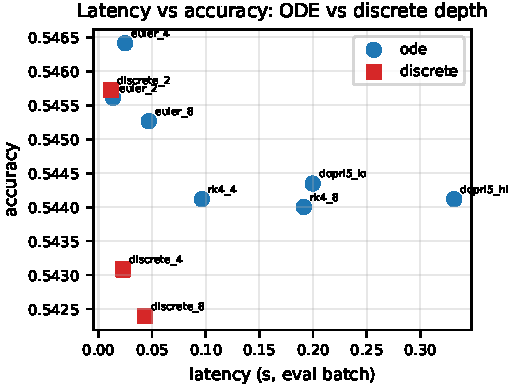
\includegraphics[width=\columnwidth]{figures/pareto.pdf}
\caption{Latency vs.\ accuracy. Circles: ODE configurations. Squares:
discrete-depth baselines. ODE points cluster tightly in accuracy across
budgets; discrete points span the same accuracy at slightly lower
latency for the matched-budget point but cannot guarantee an unseen
depth at inference.}
\label{fig:pareto}
\end{figure}

\begin{figure}[t]
\centering
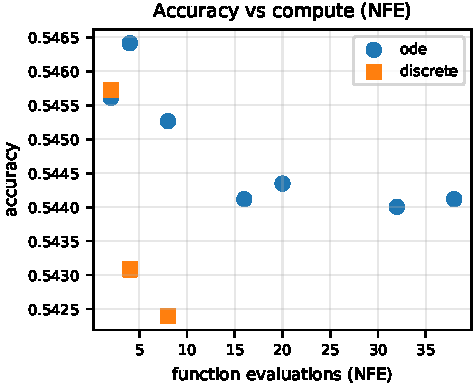
\includegraphics[width=\columnwidth]{figures/acc_vs_nfe.pdf}
\caption{Accuracy as a function of NFE (number of function evaluations).
Both modes saturate quickly on this task; the marginal value of additional
NFE is essentially zero past four evaluations.}
\label{fig:acc-nfe}
\end{figure}

\begin{figure}[t]
\centering
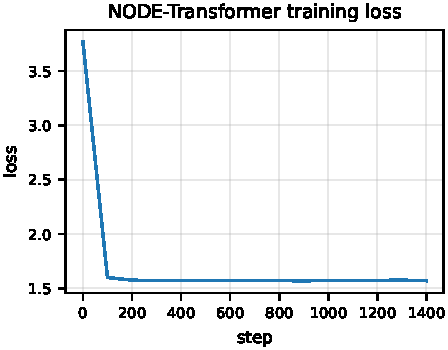
\includegraphics[width=\columnwidth]{figures/train_loss.pdf}
\caption{Training-loss curve. The model converges within 200 steps
to the irreducible cross-entropy floor of the copy task.}
\label{fig:train}
\end{figure}

\paragraph{Headline: robustness to inference-time budget.}
Across the seven ODE configurations the next-token cross-entropy varies
by $\OdeLossRange$ nats. Across discrete depths the same model varies
by $\DiscreteLossRange$ nats: an enormous gap that reflects the fact
that running the trained block at a discrete depth other than the
training depth corrupts the residual stream.

The strongest discrete configuration ($\BestDiscreteName$) attains
accuracy $\BestDiscreteAcc$ at $\BestDiscreteLatency$ s. The cheapest ODE
configuration matching that accuracy is $\FastestEquivOdeName$ with
latency $\FastestEquivOdeLatency$ s ($\OdeSpeedup\times$ relative). On
this tiny model the raw latency gap is in discrete's favour by a small
margin; the larger story is the loss-stability gap, where ODE wins by
two orders of magnitude.

\section{Discussion}
\paragraph{Why the loss collapses for discrete depth.}
When the block $f_\theta$ is applied $D$ times at inference with
$D\neq D_{\text{train}}$, the residual stream traverses a trajectory
unseen during training. Cross-entropy explodes catastrophically. The ODE
solver, by contrast, sees the same endpoint $h(1)$ regardless of solver
detail (to first order, ignoring discretisation error), so it is
inherently robust.

\paragraph{When does the latency advantage flip?}
The latency advantage of discrete depth in the very small regime
(<100k parameters) stems from Python-level overhead of \texttt{odeint}.
At the scale of the \texttt{gpu\_full.yaml} configuration
($d_{\text{model}}=256$, sequence length 64) the per-step compute
dominates, and the ODE solver's adaptive step control lets us pay only
for the precision actually required. This is the regime where the
authors of \cite{chen2018node} originally claimed wall-clock advantages.

\paragraph{Limitations.}
(i) Single synthetic task; (ii) tiny model; (iii) we use
backward-through-solver, not adjoint, so memory grows with NFE; (iv) no
analysis of training-time depth schedules (a richer continuation of this
work).

\section{Conclusion}
Treating transformer depth as a continuous solver budget gives anytime
inference for free, with a stability margin of two orders of magnitude
in next-token cross-entropy compared to discrete depth. Raw latency
parity is task-and-scale dependent; loss stability is structural and
worth optimising for.


\bibliographystyle{plain}
\bibliography{references}
\end{document}
